%!TEX root = ../dissertation.tex
%--------------------------------------------------
% \begin{savequote}[75mm]
% 
% %\qauthor{Firstname lastname}
% \end{savequote}
%-------------------------------------------------- 

\chapter{Diversity and evolution of the transposable element repertoire
in insects} \label{cha:mobilome}

This chapter has been submitted for publication in \emph{BMC
Evolutionary Biology}.

\noindent Authors: Malte Petersen, David Armisén, Richard A. Gibbs, Lars Hering,
Abderrahman Khila, Georg Mayer, Stephen Richards, Oliver Niehuis, and
Bernhard Misof

\section{Introduction}\label{mobilome-introduction}

Repetitive elements, including transposable elements (TEs), are a major
sequence component of eukaryote genomes. In vertebrate genomes, for
example, the TE content varies from 6 \% in the pufferfish
\emph{Tetraodon nigroviridis} to more than 55 \% in the zebrafish
\emph{Danio rerio} \citep{Chalopin2015}. More than 45 \% of the human
genome \citep{deKoning2011} consist of TEs. In plants, TEs are even more
prevalent: up to 90 \% of the maize (\emph{Zea mays}) genome is covered
by TEs \citep{SanMiguel1996}. In insects, the genomic portion of TEs ranges
from as little as 1 \% in the antarctic midge \citep{Kelley2014} to as
large as 65 \% in the migratory locust \citep{Wang2014}.

TEs are known as ``jumping genes'' and traditionally viewed as selfish
parasitic nucleotide sequence elements propagating in genomes with
mainly deleterious or at least neutral effects on host fitness
\citep{Mackay1989,Pasyukova2004} (reviewed in \citet{Barron2014}). Due to their
propagation in the genome, TEs are thought to have a considerable
influence on the evolution of the host's genome architecture. By
transposing into, for example, host genes or regulatory sequences, TEs
can disrupt coding sequences or gene regulation, and/or provide hot
spots for ectopic (non-homologous) recombination that may induce
chromosomal rearrangements in the host genome such as deletions,
duplications, inversions, and translocations \citep{Burns2012}. For
example, the shrinkage of the Y chromosome in the fruit fly
\emph{Drosophila melanogaster}, which consists mostly of TEs, is thought
to be caused by such intrachromosomal rearrangements induced by ectopic
recombination \citep{Adams2000,Kent2017}. As such potent agents for mutation,
TEs are also responsible for cancer and genetic diseases in humans and
other organisms \citep{Vorechovsky2009,Chenais2015,Hancks2016}.

Despite the potential deleterious effects of their activity on gene
regulation, there is growing evidence that TEs can also be drivers of
genomic innovation that confer selective advantages to the host
\citep{Casola2007,Gonzalez2008}. For example, it is well documented that the frequent
cleavage and rearrangement of DNA strands induced by TE insertions
provides a source of sequence variation to the host genome, or that by a
process called molecular domestication of TEs, host genomes derive new
functional genes and regulatory networks
\citep{Feschotte2008,Bohne2008,Santos2014}.
Furthermore, many exons have been \emph{de novo}-recruited from TE
insertions in coding sequences of the human genome \citep{Zhang2006}.
In insects, TE insertions have played a pivotal role in the acquisition
of insecticide resistance \citep{Chen2007,Itokawa2010,Gahan2001}, as well as in the rewiring
of a regulatory network that provides dosage compensation
\citep{Ellison2013}, or the evolution of climate adaptation
\citep{Gonzalez2010,Kim2014}.



TEs are classified depending on their mode of transposition. Class I
TEs, also known as retrotransposons, transpose via an RNA-mediated
mechanism that can be circumscribed as ``copy-and-paste''. They are
further subdivided into long terminal repeat (LTR) retrotransposons and
non-LTR retrotransposons. Non-LTR retrotransposons include long and
short interspersed nuclear elements (LINEs and SINEs)
\citep{Malik1999,Eickbush2008}. Whereas LTR retrotransposons and LINEs encode a
reverse transcriptase, the non-autonomous SINEs rely on the
transcriptional machinery of autonomous elements, such as LINEs, for
mobility. Frequently found LTR retrotransposon families in eukaryote
genomes include Ty3/Gypsy, which was originally described in
\emph{Arabidopsis thaliana} \citep{Marin2000}, Ty1/Copia
\citep{Flavell1992}, as well as BEL/Pao \citep{delaChaux2011}.

In Class II TEs, also termed DNA transposons, the transposition is
DNA-based and does not require an RNA intermediate. Autonomous DNA
transposons encode a transposase enzyme and move via a ``cut-and-paste''
mechanism. During replication, terminal inverted repeat (TIR)
transposons and Crypton-type elements cleave both DNA strands
\citep{Wicker2007}. Helitrons, also known as rolling-circle (RC)
transposons due to their characteristic mode of transposition
\citep{Kapitonov2001}, and the self-synthesizing Maverick/Polinton elements
\citep{Krupovic2016} cleave a single DNA strand in the process of
replication. Both Helitron and Maverick/Polinton elements occur in
autonomous and non-autonomous versions \citep{Kapitonov2006,Kapitonov2007}, the latter of
which do not encode all proteins necessary for transposition. Helitrons
are the only Class II transposons that do not cause a flanking target
site duplication when they transpose. Class II also encompasses other
non-autonomous DNA transposons such as miniature inverted TEs (MITEs)
\citep{Shirasawa2012}, which exploit and rely on the transposase mechanisms
of autonomous DNA transposons to replicate.

Previous reports on insect genomes describe the composition of TE
families in insect genomes as a mixture of insect specific TEs and TEs
common to metazoa \citep{Feschotte2007,Maumus2015,Chuong2016}. Overall, surprisingly little
effort has been put into characterizing TE sequence families and TE
compositions in insect genomes in large-scale comparative analyses
encompassing multiple taxonomic orders to paint a picture of the insect
TE repertoire. Dedicated comparative analyses of TE composition have
been conducted on species of mosquitoes \citep{Neafsey2015}, of
drosophilid flies \citep{Sessegolo2016}, and of \emph{Macrosiphini}
(aphids) \citep{Bouallegue2017}. Despite these efforts in characterizing TEs
in insect genomes, still little is known about the diversity of TEs in
insect genomes, owed in part to the huge insect species diversity and to
the lack of a standardized analysis that allows comparisons across
taxonomic orders. While this lack of knowledge is due to the low
availability of sequenced insect genomes in the past, efforts such as
the i5k initiative \citep{Robinson2011} have helped to increase the number
of genome sequences from previously unsampled insect taxa. With this
denser sampling of insect genomic diversity available, it now seems
possible to comprehensively investigate the TE diversity among major
insect lineages.

Here, we present the first exhaustive analysis of the distribution of TE classes in a sample representing half of the currently classified insect orders and using standardized comparative methods implemented in recently developed software packages.
Our results show similarities in TE family diversity and abundance among the investigated insect genomes, but also profound differences in TE activity even among closely related species.

\section{Materials and methods}\label{materials-and-methods}

\subsection{Genomic data sets}\label{genomic-data-sets}

We downloaded genome assemblies of 42 arthropod species from NCBI
GenBank at \url{ftp.ncbi.nlm.nih.gov/genomes} (last accessed 2014-11-26;
supplementary table \ref{tab:urls} on page \pageref{tab:urls}) as well
as the genome assemblies of 31 additional species from the i5k FTP
server at \url{ftp.hgsc.bcm.edu/I5K-pilot} (last accessed 2016-07-08;
supplementary table \ref{tab:urls}). Our taxon sampling includes 21
dipterans, four lepidopterans, one trichopteran, five coleopterans, one
strepsipteran, 14 hymenopterans, one psocodean, six hemipterans, one
thysanopteran, one blattodean, one isopteran, one orthopteran, one
ephemeropteran, one odonate, one archaeognathan, and one dipluran. As
outgroups we included three crustaceans, one myriapod, six chelicerates,
and one onychophoran.

\subsection{Construction of species-specific repeat libraries and TE
annotation in the
genomes}\label{construction-of-species-specific-repeat-libraries-and-te-annotation-in-the-genomes}

We compiled species-specific TE libraries using automated annotation
methods. RepeatModeler Open-1.0.8 \citep{Smit2015} was employed to
cluster repetitive \emph{k}-mers in the assembled genomes and infer
consensus sequences. These consensus sequences were classified using a
reference-based similarity search in RepBase Update 20140131
\citep{Jurka2005}. The entries in the resulting repeat libraries were
then searched for using nucleotide BLAST in the NCBI nr database
(downloaded 2016-03-17 from
\href{ftp://ftp.ncbi.nlm.nih.gov/blast/db}{ftp.ncbi.nlm.nih.gov/blast/db})
to verify that the included consensus sequences are indeed TEs and not
annotation artifacts. Repeat sequences that were annotated as
``unknown'' and that resulted in a BLAST hit for known TE proteins such
as reverse transcriptase, transposase, integrase, or known TE domains
such as gag/pol/env, were kept and considered unknown TE nucleotide
sequences; but all other ``unknown'' sequences were not considered TE
sequences and therefore removed. The filter patterns are listed in
supplementary table \ref{tab:patterns} on page \pageref{tab:patterns}.
The filtered repeat library was combined with the Metazoa-specific
section of RepBase version 20140131 and subsequently used with
RepeatMasker 4.0.5 \citep{Smit2015a} to annotate TEs in the genome
assemblies.

\subsection{Validation of Alu
presence}\label{validation-of-alu-presence}

To exemplarily validate our annotation, we selected the SINE Alu, which
was previously only identified in primates \citep{Kriegs2007}. We
retrieved a Hidden Markov model (HMM) profile for the AluJo subfamily
from the repeat database Dfam \citep{Hubley2015} and used the HMM to
search for Alu copies in the genome assemblies. We extracted the hit
nucleotide subsequences from the assemblies and inferred a multiple
nucleotide sequence alignment with the canonical Alu nucleotide sequence
from Repbase \citep{Jurka2005}.

\subsection{Genomic TE coverage and correlation with genome
size}\label{genomic-te-coverage-and-correlation-with-genome-size}

We used the tool ``one code to find them all'' \citep{Bailly-Bechet2014}
on the RepeatMasker output tables to calculate the genomic proportion of
annotated TEs. ``One code to find them all'' is able to merge entries
belonging to fragmented TE copies to produce a more accurate estimate of
the genomic TE content and especially the copy numbers. To test for a
relationship between genome assembly size and TE content, we applied a
linear regression model and tested for correlation using the Spearman
rank sum method. To see whether the genomes of holometabolous insects
are different than the genomes of hemimetabolous insects in TE content,
we tested for an effect of the taxa using their mode of metamorphosis as
a three-class factor: Holometabola (all holometabolous insect species),
non-Eumetabola (all non-holometabolous hexapod species, with the
exception of Hemiptera, Thysanoptera, and Psocodea;
\citet{Beutel2013}), and Acercaria (Hemiptera, Thysanoptera, and
Psocodea). We also tested for a potential phylogenetic effect on the
correlation between genome size and TE content with the phylogenetic
independent contrasts (PIC) method proposed by \citet{Felsenstein1985}
using the ape package \citep{Paradis2004} within R \citep{RCoreTeam2017}





\subsection{Kimura distance-based TE age
distribution}\label{kimura-distance-based-te-age-distribution}

We used intra-family TE nucleotide sequence divergence as a proxy for
intra-family TE age distributions. Sequence divergence was calculated as
intra-family Kimura distances (rates of transitions and transversions)
using the specialized helper scripts from the RepeatMasker 4.0.5
package. The tools compute the Kimura distance between each annotated TE
copy and the consensus sequence of the respective TE family, and provide
the data in tabular format for processing. When plotted (Fig.
\ref{fig:landscapes} on page \pageref{fig:landscapes}), a peak in the
distribution shows the genomic coverage of the TE copies with that
specific Kimura distance to the repeat family consensus. Thus, a large
peak with high Kimura distance would indicate a group of TE copies with
high sequence divergence due to genetic drift or other processes.  The
respective TE copies are likely older than copies associated with a peak
at low Kimura distance. We used the Kimura distances without correction
for CpG pairs since TE DNA methylation is clearly absent in
holometabolous insects and insufficiently described in hemimetabolous
insects \citep{Glastad2014}.  All TE age distribution landscapes were
inferred from the data obtained by annotating the genomes with \emph{de
novo}-generated species-specific repeat libraries.

\section{Results}\label{results}

\subsection{Diversity of TE content in arthropod
genomes}\label{diversity-of-te-content-in-arthropod-genomes}

TE content varies greatly among the analyzed species (Fig.
\ref{fig:te-coverage} on page \pageref{fig:te-coverage}, supplemental
table \ref{tab:coverage} on page \pageref{tab:coverage}) and differs
even between species belonging the same order. In the insect order
Diptera, for example, the TE content varies from around 55 \% in the
yellow fever mosquito \emph{Aedes aegypti} to less than 1 \% in
\emph{Belgica antarctica}. Even among closely related \emph{Drosophila}
species, the TE content ranges from 40 \% (in \emph{D. ananassae}) to 10
\% (in \emph{D. miranda} and \emph{D.  simulans}). The highest TE
content (60 \%) was found in the large genome (6.5 Gbp) of the migratory
locust \emph{Locusta migratoria} (Orthoptera), while the smallest known
insect genome, that of the antarctic midge \emph{B. antarctica}
(Diptera, 99 Mbp), was found to contain less than 1 \% TEs. The TE
content of the majority of the genomes was spread around a median of
24.4 \% with a standard deviation of 12.5 \%.

\begin{figure}[h!]
\begin{center}
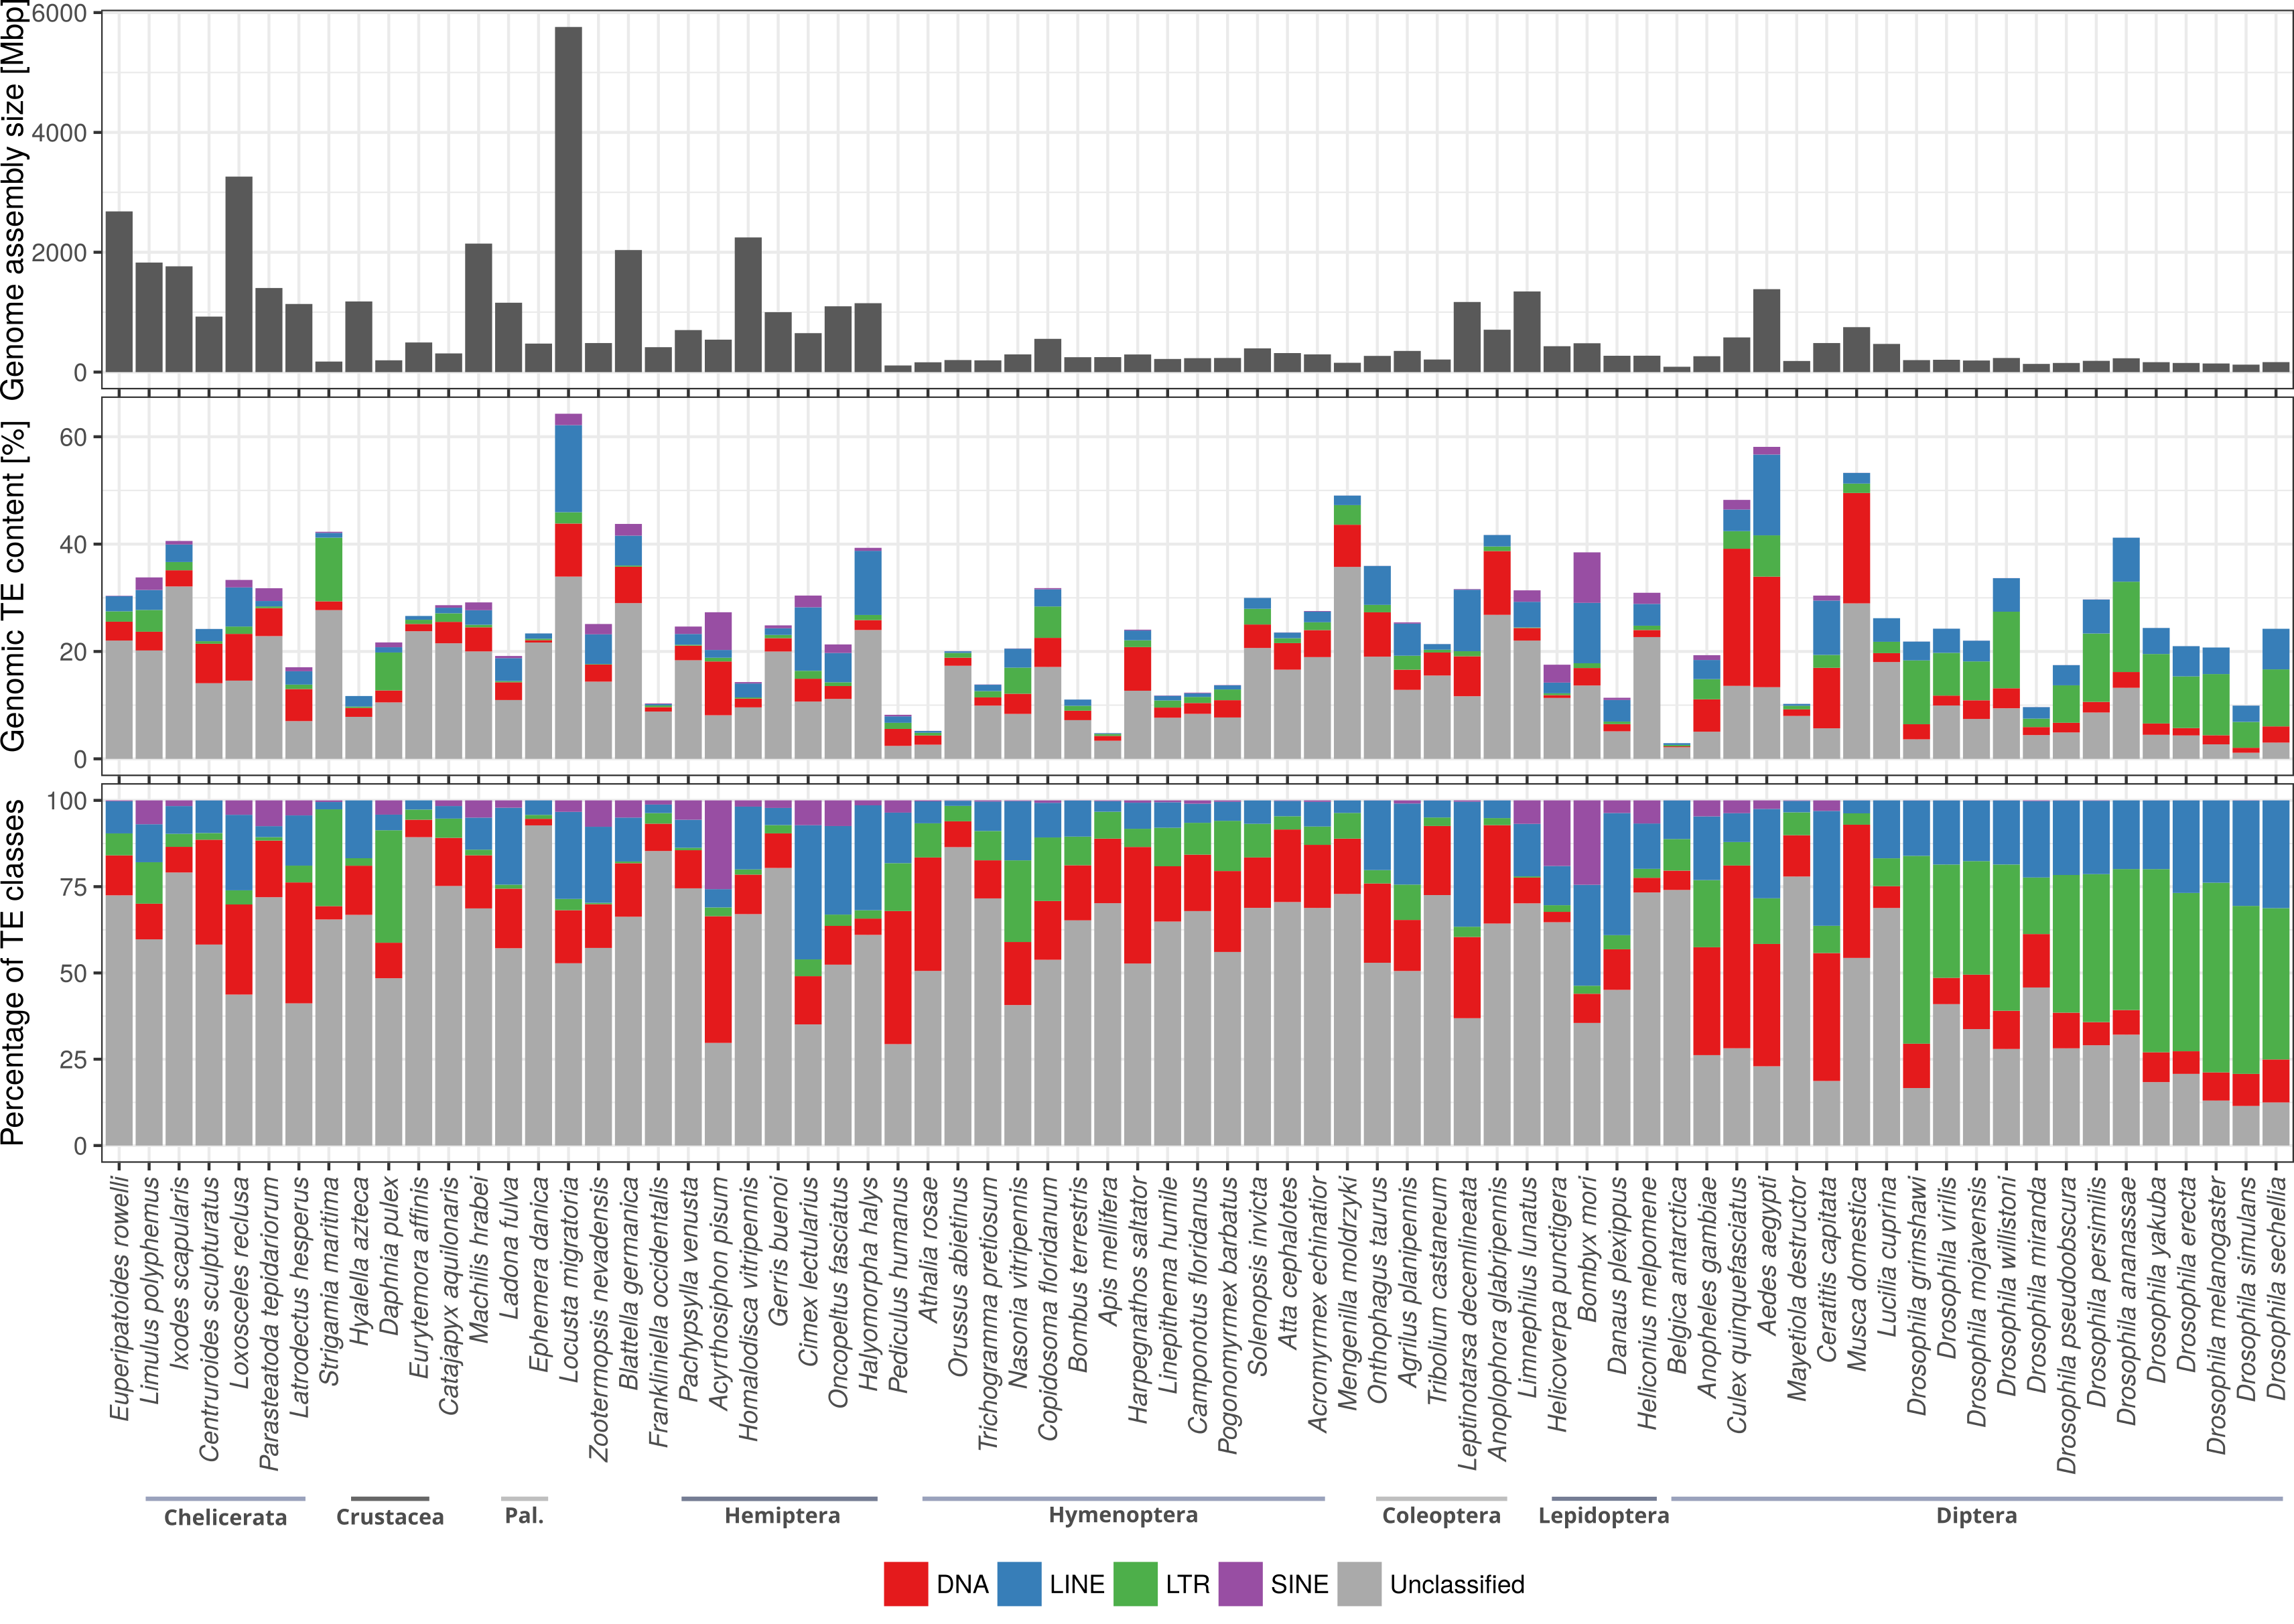
\includegraphics[width=\textwidth]{te-coverage-in-insect-genomes-both}
\caption[TE coverage (absolute and relative) in arthropod
genomes]{{Genome assembly size, total amount and relative proportion of
DNA transposons, LTR, LINE and SINE retrotransposons in arthropod
genomes and a representative of Onychophora as an outgroup. Also shown
is the genomic proportion of unclassified/uncharacterized repetitive
elements.  Pal., Palaeoptera%
}}%
\label{fig:te-coverage}%
\end{center}
\end{figure}

\subsection{Relative contribution of different TE types to arthropod
genome
sequences}\label{relative-contribution-of-different-te-types-to-arthropod-genome-sequences}

We assessed the relative contribution of the major TE groups (LTR, LINE,
SINE retrotransposons, and DNA transposons) to the arthropod genome
composition (Fig. \ref{fig:te-coverage} on page
\pageref{fig:te-coverage}). In most species, ``unclassified'' elements,
which need further characterization, represent the largest fraction.
They contribute up to 93 \% of the total TE coverage in the mayfly
\emph{Ephemera danica} or the copepod \emph{Eurytemora affinis}.
Unsurprisingly, in most investigated \emph{Drosophila} species the
unclassifiable elements comprise less than 25 \% and in \emph{D.
simulans} only 11 \% of the entire TE content, likely because the
\emph{Drosophila} genomes are well annotated and most of their content
is known (in fact, many TEs were first found in representatives of
\emph{Drosophila}). Disregarding these unclassified TE sequences, LTR
retrotransposons dominate the TE content in representatives of Diptera,
in some cases contributing around 50 \% (e.g., in \emph{D. simulans}).
In Hymenoptera, on the other hand, DNA transposons are more prevalent,
such as 35.25 \% in Jerdon's jumping ant \emph{Harpegnathos saltator}.
LINE retrotransposons are represented with up to 39.3 \% in Hemiptera
and Psocodea (\emph{Acyrthosiphon pisum} and \emph{Cimex lectularius}),
with the exception of the human body louse \emph{Pediculus humanus},
where DNA transposons contribute 44.43 \% of the known TE content. SINE
retrotransposons were found in all insect orders, but they contributed
less than 10 \% of the genomic TE content in any taxon in our sampling,
with the exception of \emph{Helicoverpa punctigera} (18.48 \%),
\emph{Bombyx mori} (26.38 \%), and \emph{A. pisum} (27.11). In some
lineages, such as Hymenoptera and most dipterans, SINEs contribute less
than 1 \% to the TE content, whereas in Hemiptera and Lepidoptera the
SINE coverage ranges from 0.08 \% to 26.38 \% (Hemiptera) and 3.35 \% to
26.38 \% (Lepidoptera). Note that these numbers are likely higher and
many more DNA, LTR, LINE, and SINE elements may be obscured by the large
``unclassified'' portion.

\subsection{Contribution of TEs to arthropod genome
size}\label{contribution-of-tes-to-arthropod-genome-size}

We assessed the TE content, that is, the ratio of TE versus non-TE
nucleotides in the genome assembly, in 62 hexapod species as well as an
outgroup of 10 non-insect arthropods and a representative of Onychophora
(velvet worms). We tested whether there was a relationship between TE
content and genome assembly size, and found a positive correlation (Fig.
\ref{fig:te-coverage-vs-genome-size} on page
\pageref{fig:te-coverage-vs-genome-size} and supplemental table
\ref{tab:coverage} on page \pageref{tab:coverage}). This correlation is
statistically significant (Spearman's rank sum test, \(\rho = 0.495\),
\(p \lll 0.005\)). Genome size is significantly smaller in
holometabolous insects than in non-holometabolous insects (one-way
ANOVA, \(p = 0.0001\)). Using the \texttt{ape} package v. 4.1
\citep{Paradis2004} for R \citep{RCoreTeam2017}, we tested for
correlation between TE content and genome size using phylogenetically
independent contrasts (PIC) \citep{Felsenstein1985}. The test confirmed
a significant positive correlation (Pearson product-moment correlation,
\(\rho = 0.497\), \(p = 0.0001\), corrected for phylogeny using PIC)
between TE content and genome size. Additionally, genome size is
correlated with TE diversity, that is, the number of different TE
superfamilies found in a genome (Spearman, \(\rho = 0.712\), \(p \lll
0.005\)); this is also true under PIC (Pearson, \(\rho = 0.527\), \(p
\lll 0.005\); Fig. \ref{fig:te-families-vs-genome-size} on page
\pageref{fig:te-families-vs-genome-size}).

\begin{figure}[h!]
\begin{center}
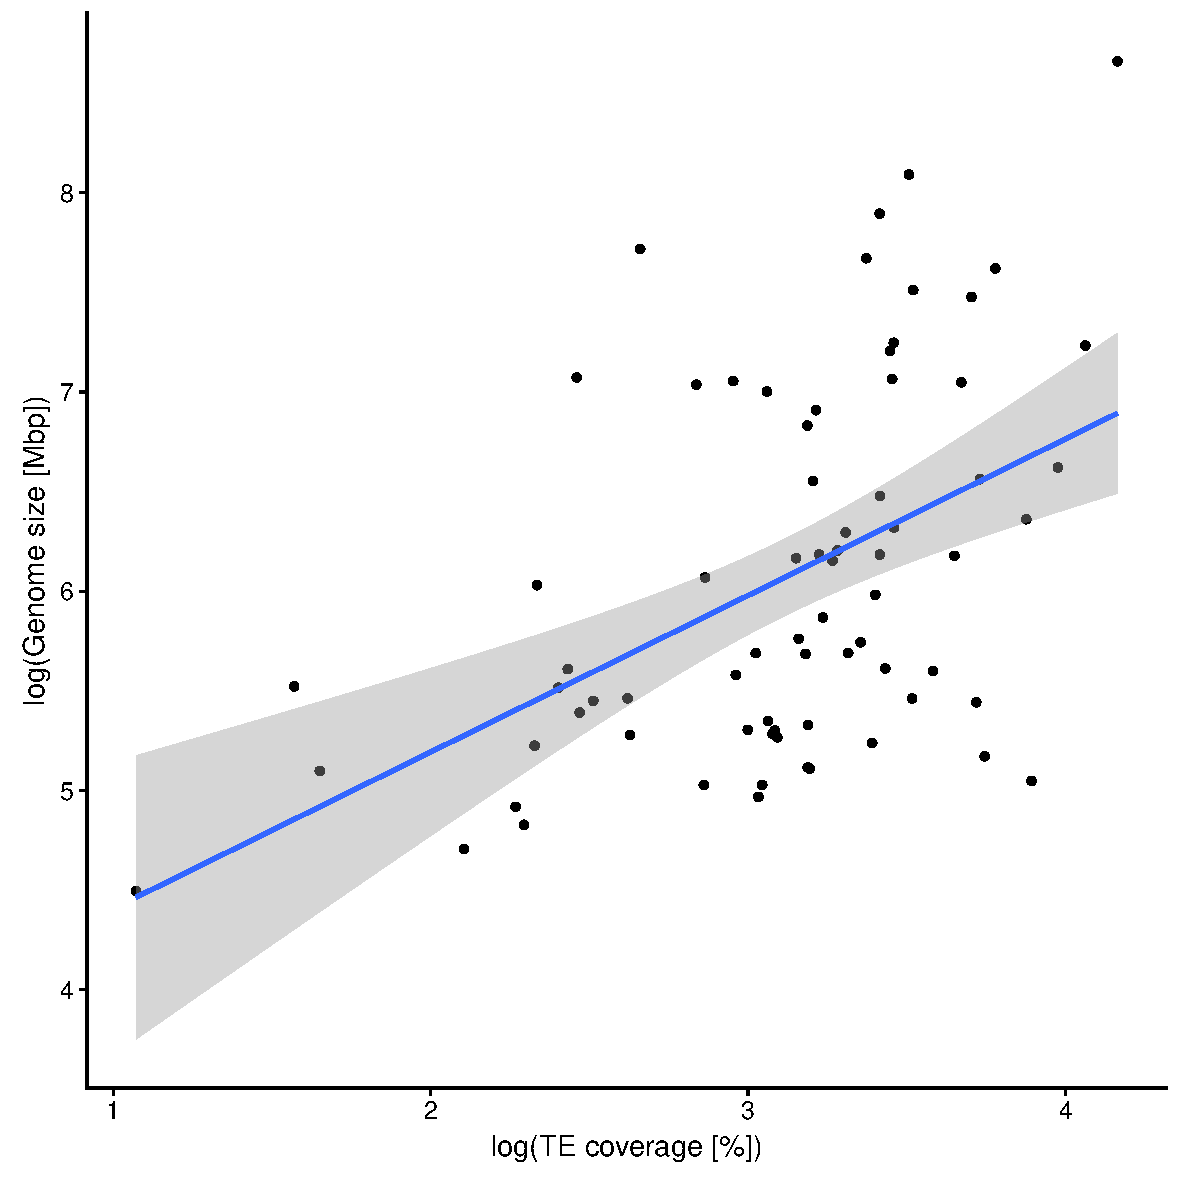
\includegraphics[width=0.60\textwidth]{te-coverage-vs-genome-size}
\caption[TE content is correlated to genome size]{{TE content in 73 arthropod genomes is positively correlated to genome
assembly size (Spearman rank correlation test, \(\rho = 0.495\),
\(p \lll 0.005\)). This correlation is also supported under
phylogenetically independent contrasts \protect\citep{Felsenstein1985} (Pearson
product moment correlation, \(\rho = 0.497\), \(p = 0.0001225\)). Dots:
Individual measurements; blue line: linear regression; grey area:
confidence interval.%
}}%
\label{fig:te-coverage-vs-genome-size}%
\end{center}
\end{figure}

\subsection{Distribution of TE superfamilies in
arthropods}\label{distribution-of-te-superfamilies-in-arthropods}

We identified almost all known TE superfamilies in at least one insect
species, and many were found to be widespread and present in all
investigated species (Fig. \ref{fig:presence-absence} on page
\pageref{fig:presence-absence}, note that in this figure, TE families
were summarized in superfamilies). Especially diverse and ubiquitous are
DNA transposon superfamilies, which represent 22 out of 70 identified TE
superfamilies. The most widespread (present in all investigated species)
DNA transposons belong to the superfamilies Academ, Chapaev and other
superfamilies in the CMC complex, Crypton, Dada, Ginger, hAT (Blackjack,
Charlie, \emph{etc.}), Kolobok, Maverick, Harbinger, PiggyBac, Helitron
(RC), Sola, TcMar (Mariner, Tigger, \emph{etc.}), and the P element
superfamily. LINE non-LTR retrotransposons are similarly ubiquitous,
though not as diverse. Among the most widespread LINEs are TEs belonging
to the superfamilies CR1, Jockey, L1, L2, LOA, Penelope, R1, R2, and
RTE. Of the LTR retrotransposons, the most widespread are in the
superfamilies Copia, DIRS, Gypsy, Ngaro, and Pao as well as endogenous
retrovirus particles (ERV). SINE elements are diverse, but show a more
patchy distribution, with only the tRNA-derived superfamily present in
all investigated species. We found elements belonging to the ID
superfamily in almost all species except the Asian long horned beetle,
\emph{Anoplophora glabripennis}, and the B4 element absent from eight
species. All other SINE superfamilies are absent in at least 13 species.
Elements from the Alu superfamily were found in 48 arthropod genomes,
for example in the silkworm \emph{Bombyx mori} (Fig.
\ref{fig:alu-in-zneva} on page \pageref{fig:alu-in-zneva}, all Alu
alignments are shown in supplemental file 1).

\begin{figure}[h!]
\begin{center}
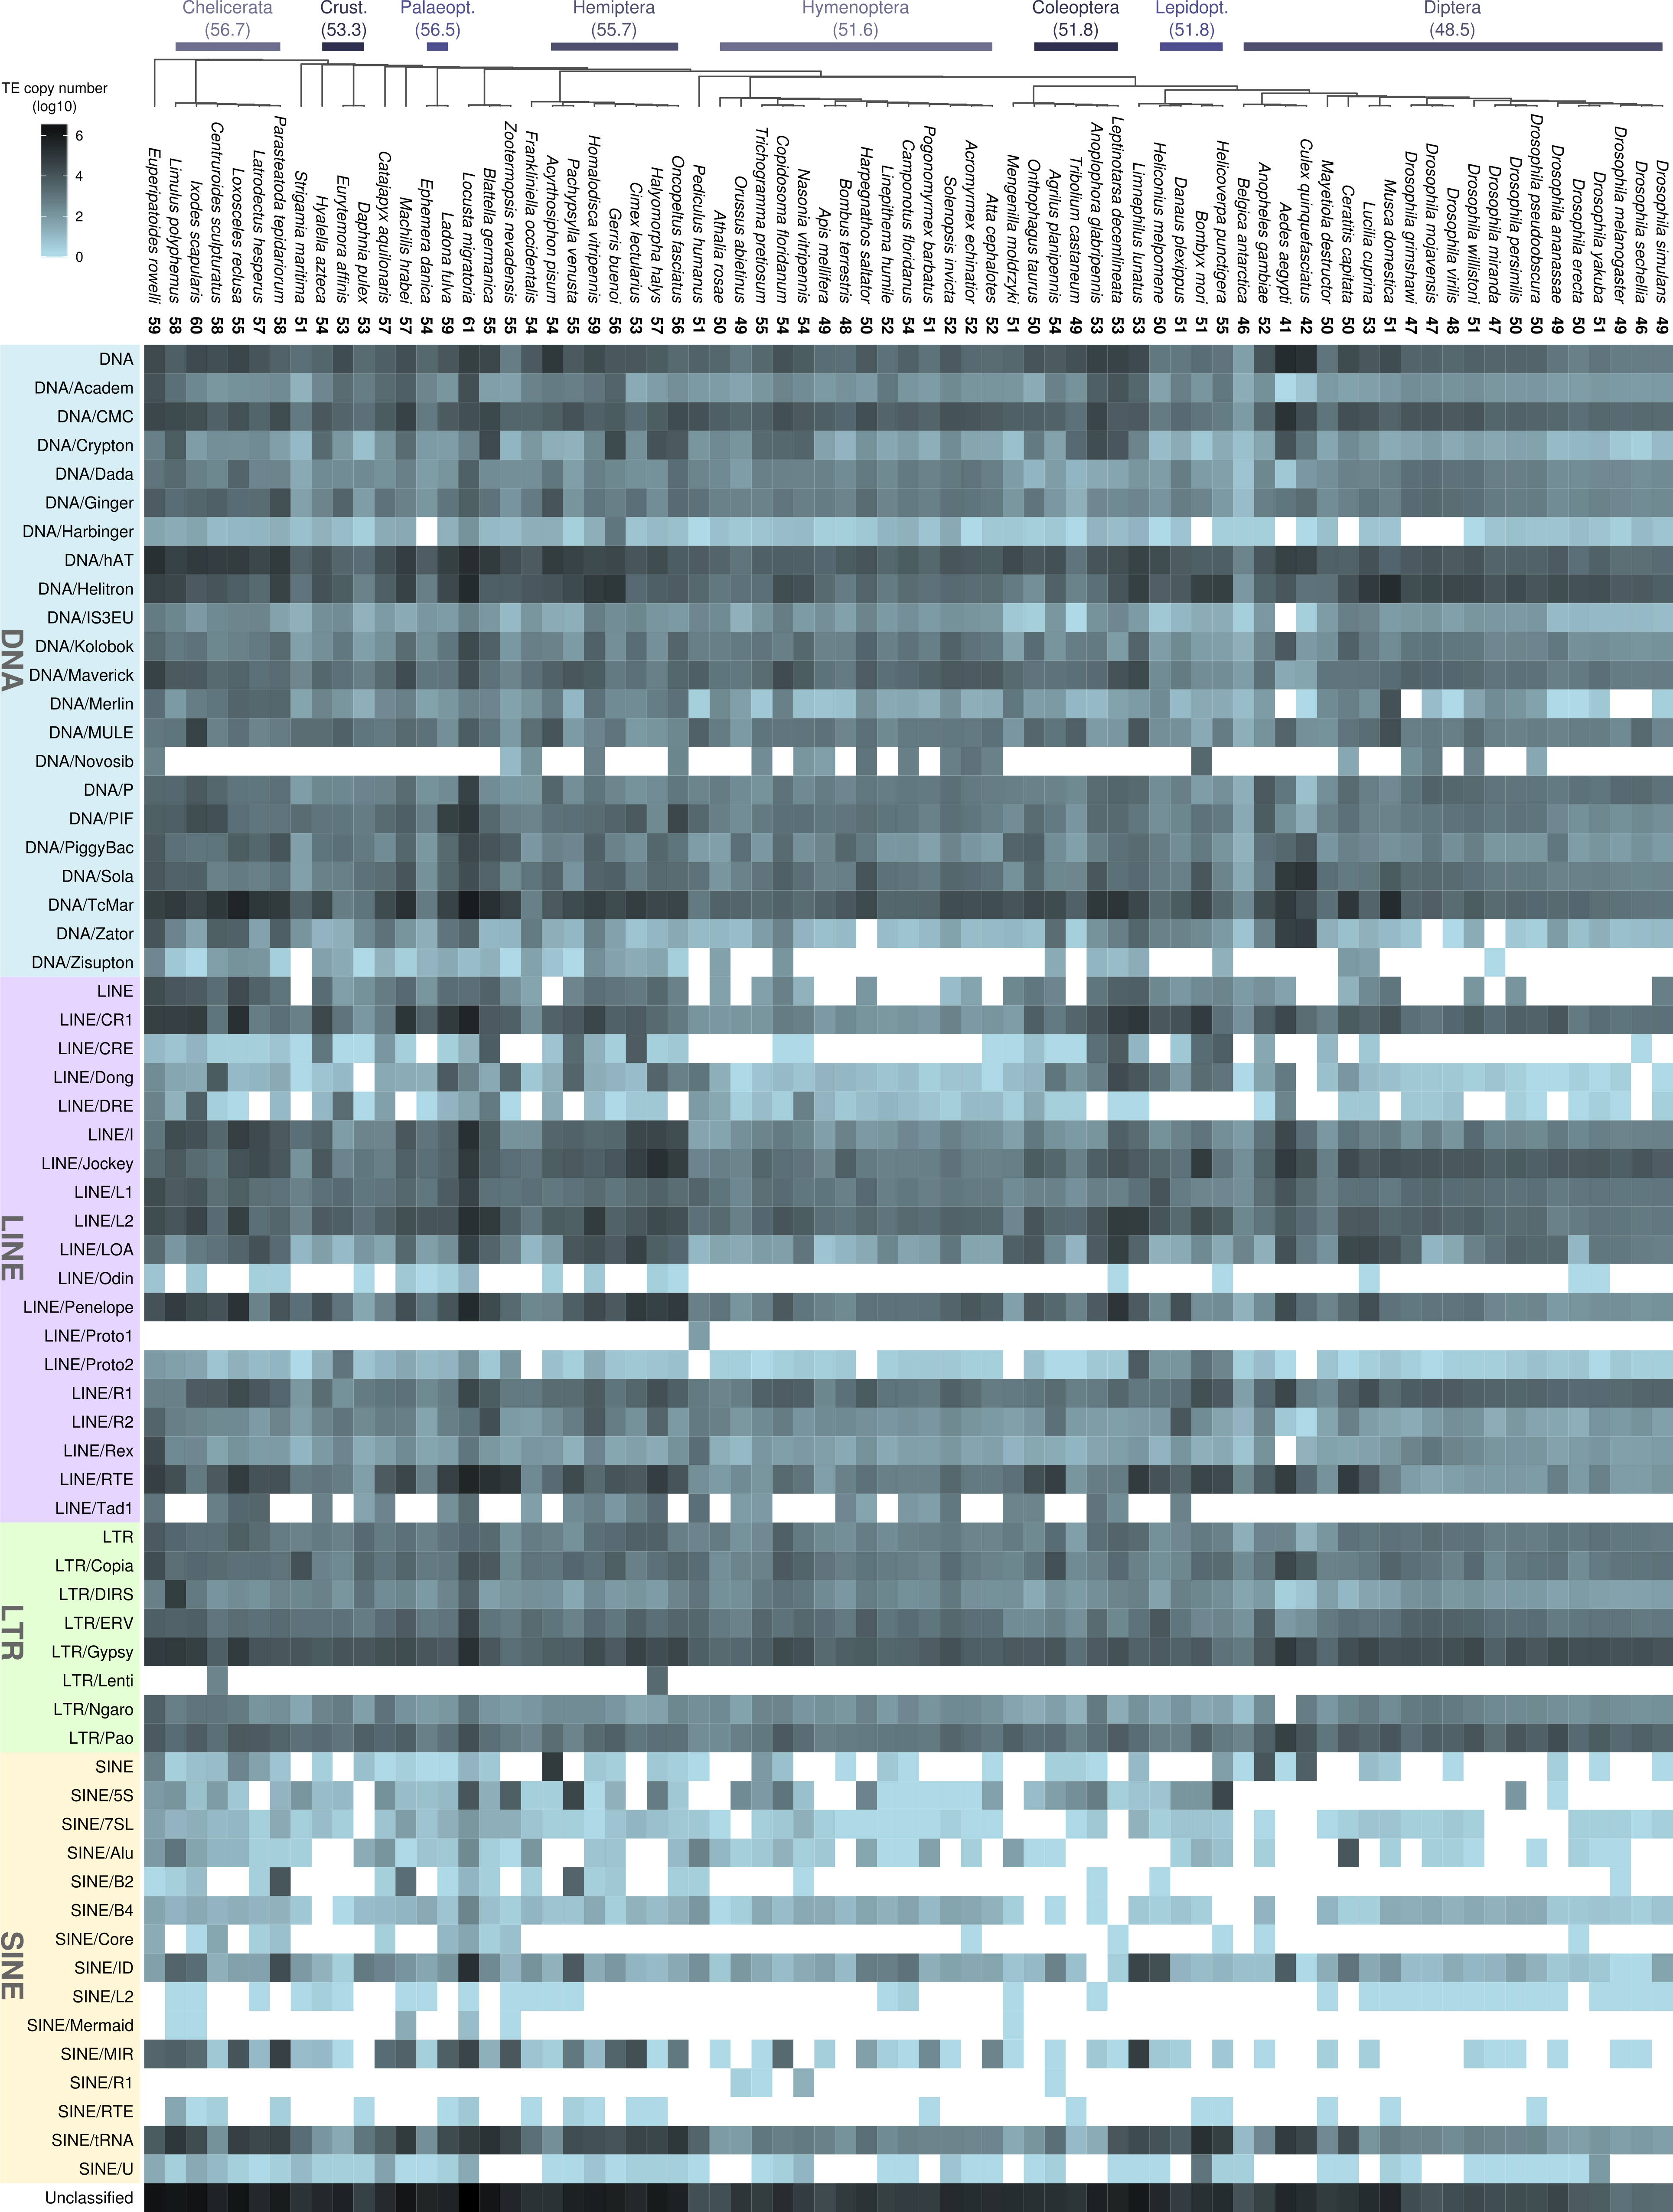
\includegraphics[height=0.91\textheight]{presence-absence-reduced-with-tree}
\caption[Presence and absence of TE superfamilies in arthropod genomes]{{TE diversity in arthropod genomes: Many known TE superfamilies were
identified in almost all insect species. Presence of TE superfamilies is
shown as filled cells with the color gradient showing the TE copy number
(log11). Empty cells represent absence of TE superfamilies. The numbers
after each species name show the number of different TE superfamilies;
numbers in parentheses below clade names denote the average number of TE
superfamilies in the corresponding taxon.%
}}%
\label{fig:presence-absence}%
\end{center}
\end{figure}

\begin{sidewaysfigure}[t]
\begin{center}
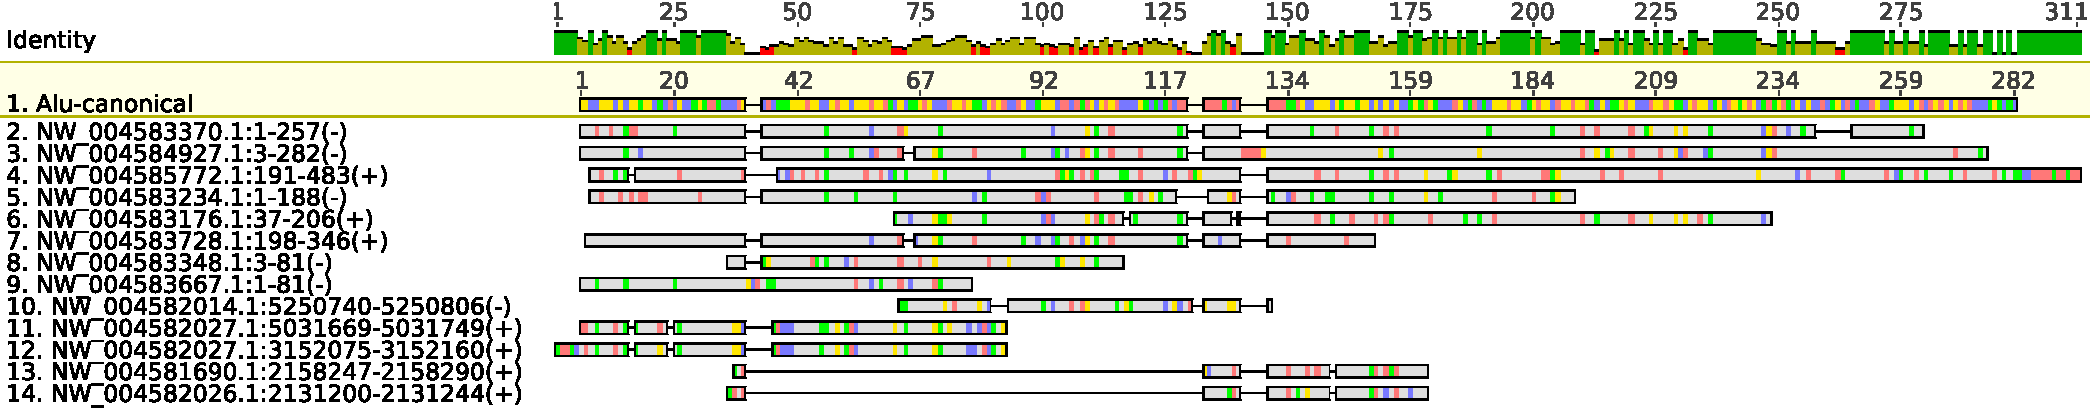
\includegraphics[width=\textwidth]{Alu-in-Zootermopsis-nevadensis}
\caption[The Alu element in the \species{Bombyx mori} genome]{{The Alu element found in \species{Bombyx mori}: Alignment of the
canonical Alu sequence from Repbase with HMM hits in the \species{B. mori}
genome assembly. Grey areas in the sequences are identical to the
canonical Alu sequence. The sequence names follow the pattern
``identifier:start-end(strand)'' Image created using Geneious version
7.1 created by Biomatters. Available from \url{https://www.geneious.com}
}}%
\label{fig:alu-in-zneva}
\end{center}
\end{sidewaysfigure}

On average, the analyzed species harbor a mean of 54.8 different TE
superfamilies, with the locust \emph{L. migratoria} exhibiting the
greatest diversity (61 different TE superfamilies), followed by the tick
\emph{Ixodes scapularis} (60), the velvet worm \emph{Euperipatoides
rowelli} (59), and the dragonfly \emph{Ladona fulva} (59). Overall,
Chelicerata have the highest average TE superfamily diversity (56.7).
The greatest diversity among the multi-representative hexapod orders was
found in Hemiptera (55.7). The mega-diverse insect orders Diptera,
Hymenoptera, and Coleoptera display a relatively low diversity of TE
superfamilies (48.5, 51.8, and 51.8, respectively). The lowest diversity
was found in \emph{A. aegypti}, with only 41 TE superfamilies.

\subsection{Lineage-specific TE presence and absence in insect
orders}\label{lineage-specific-te-presence-and-absence-in-insect-orders}

We found lineage-specific TE diversity within most insect orders. For
example, the LINE superfamily Odin is absent in all Hymenoptera studied,
whereas Proto2 was found in all Hymenoptera except in the ant \emph{H.
saltator} and in all Diptera except in \emph{C. quinquefasciatus}.
Similarly, the Harbinger DNA element superfamily was found in all
Lepidoptera except for the silkworm \emph{B. mori}. Also within
Palaeoptera (\emph{i.e.}, mayflies, damselflies, and dragonflies), the
Harbinger superfamily is absent in \emph{E. danica}, but present in all
other representatives of Palaeoptera. These clade-specific absences of a
TE superfamily may be the result of lineage-specific TE extinction
events during the evolution of the different insect orders. Note that
since a superfamily can encompass multiple different TEs, the absence of
a specific superfamily can either result from independent losses of
multiple TEs belonging to that superfamily, or a single loss if there
only was a single TE of that superfamily in the genome.

We also found TE superfamilies represented only in a single species of
an insect clade. For example, the DNA element superfamily Zisupton was
found only in the wasp \emph{Copidosoma floridanum}, but not in other
Hymenoptera, and the DNA element Novosib was found only in \emph{B.
mori}, but not in other Lepidoptera. Within Coleoptera, only the
Colorado potato beetle, \emph{Leptinotarsa decemlineata} harbors the
LINE superfamily Odin. Likewise, we found the Odin superfamily among
Lepidoptera only in the noctuid \emph{Helicoverpa punctigera}. We found
the LINE superfamily Proto1 only in \emph{Pediculus humanus} and in no
other species. These examples of clade or lineage specific occurrence of
TEs, which are absent from other species of the same order (or the
entire taxon sampling), could be the result of a horizontal transfer
from food species or a bacterial/viral infection.



\subsection{Lineage-specific TE activity during arthropod
evolution}\label{lineage-specific-te-activity-during-arthropod-evolution}

\begin{figure}[h!]
\begin{center}
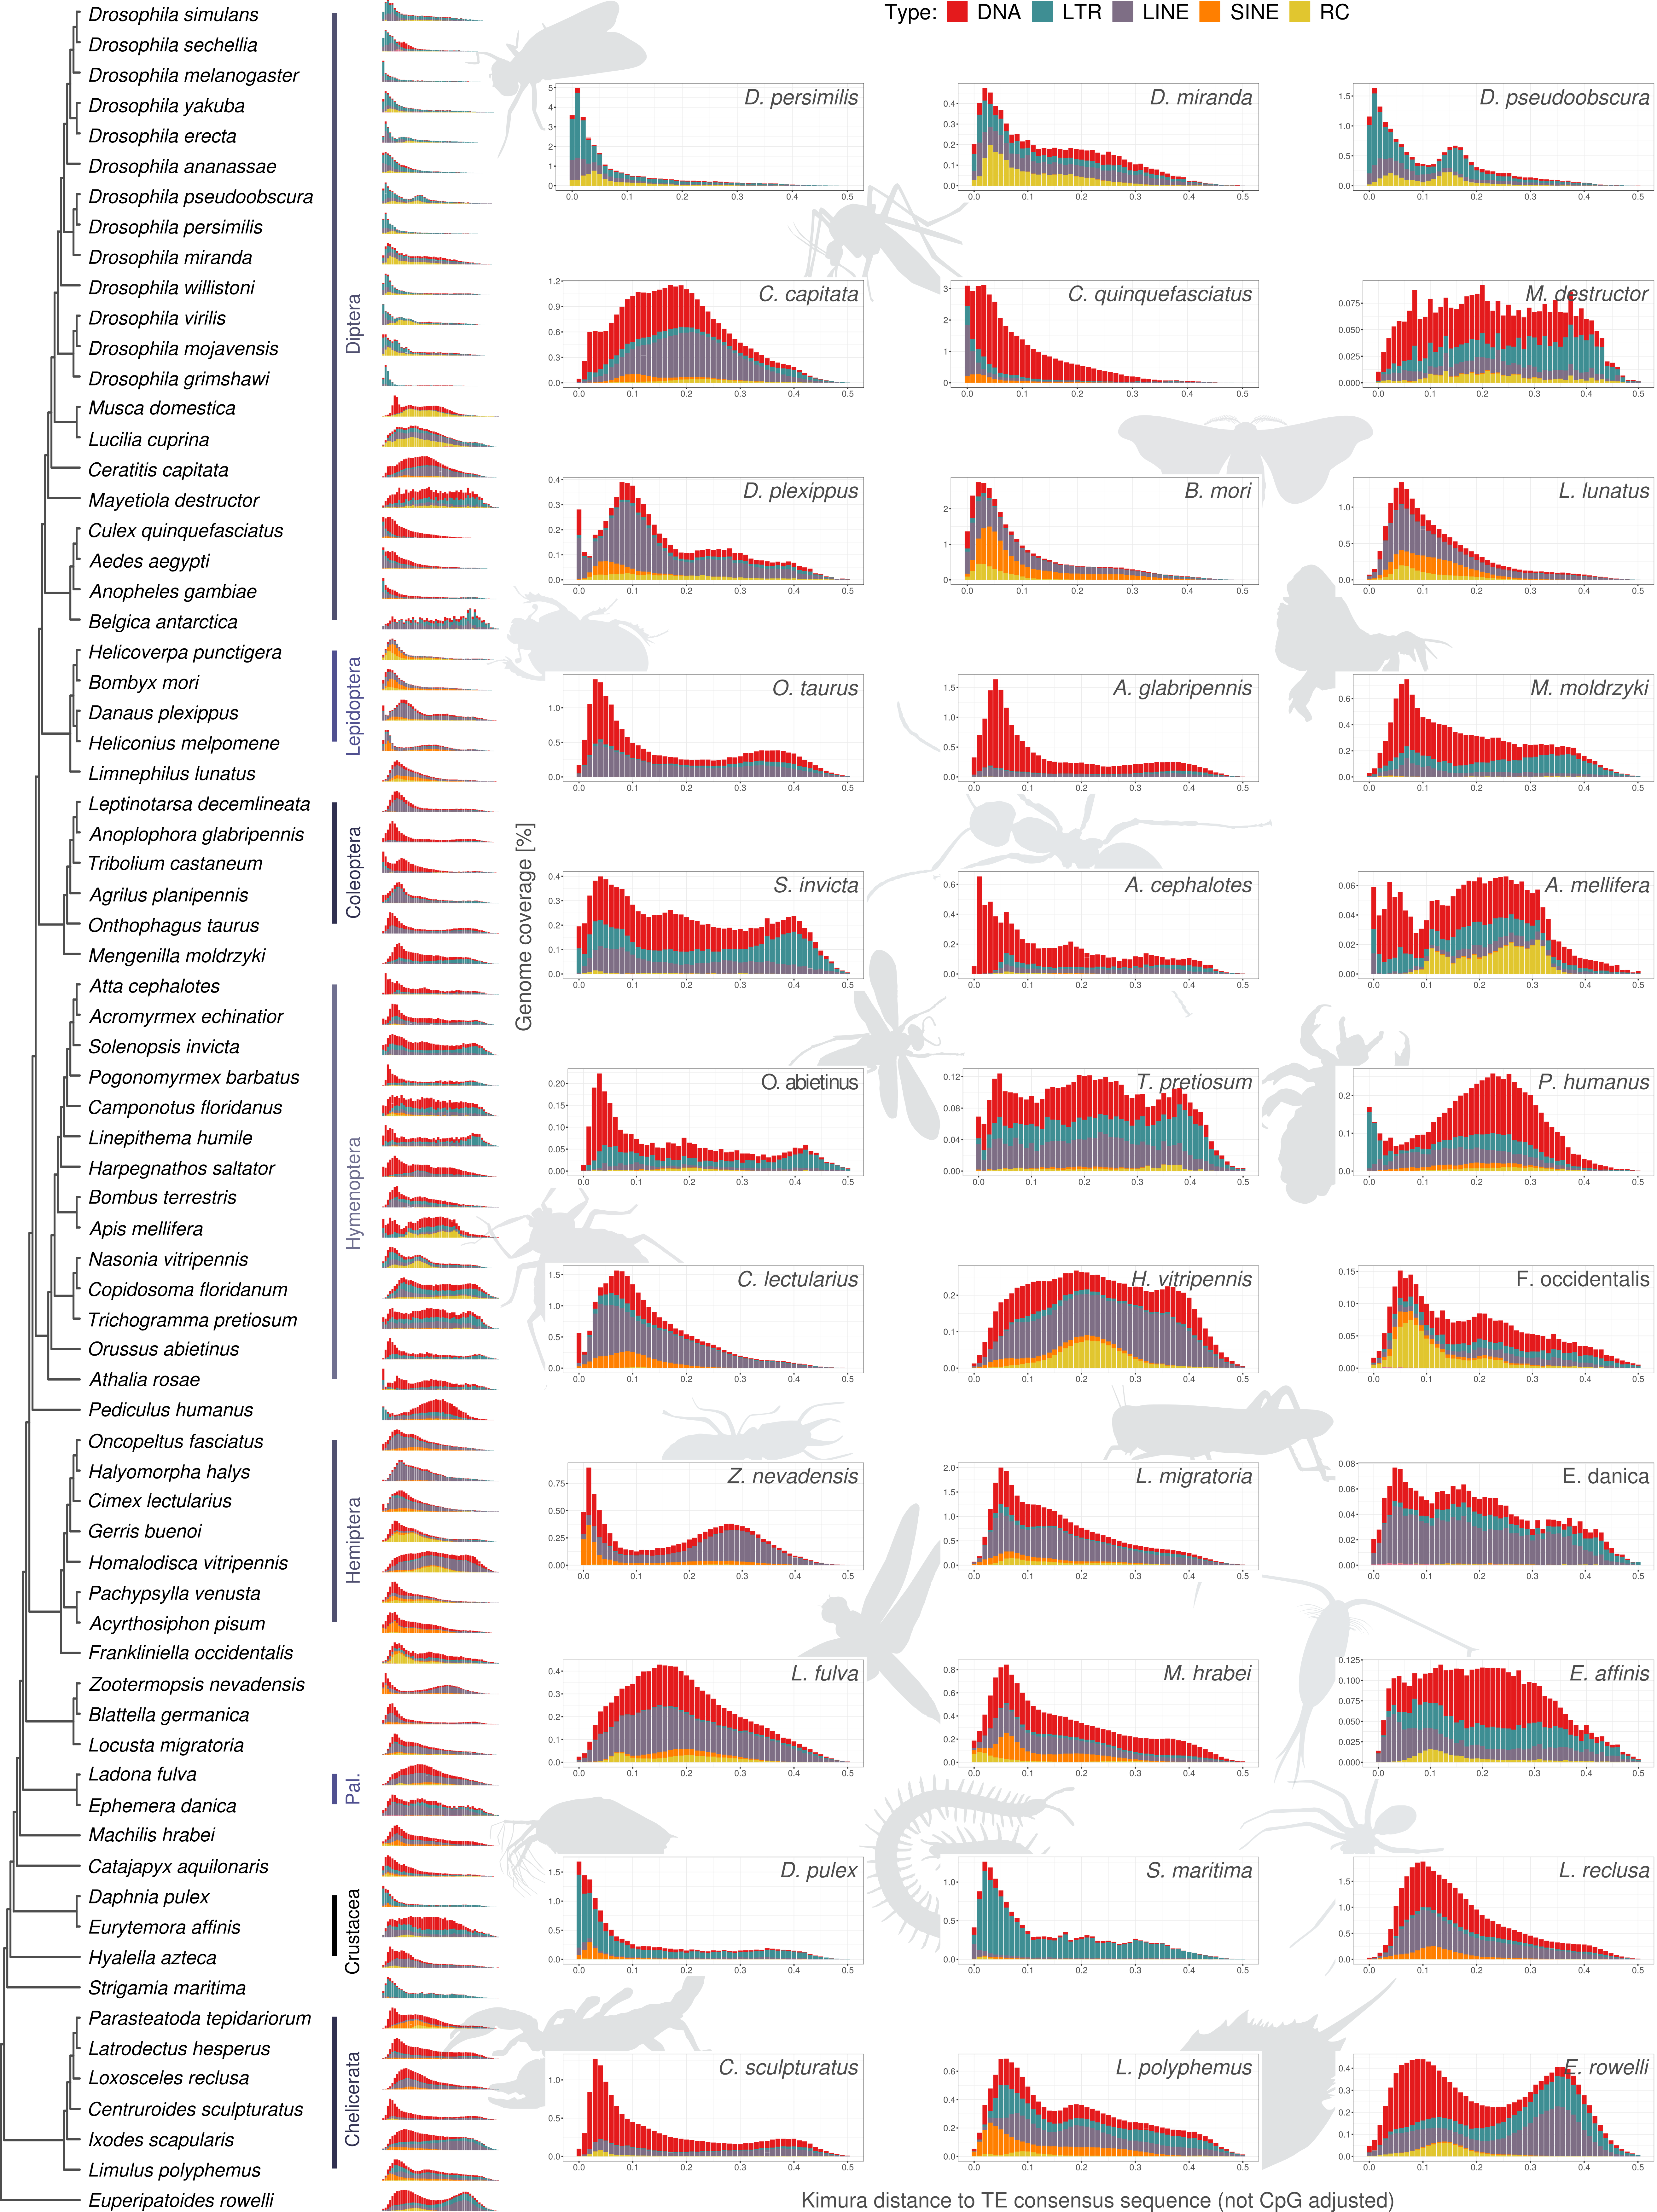
\includegraphics[height=0.93\textheight]{tree-with-landscapes-and-larger-plots}
\caption[Arthropod repeat landscapes]{{Cladogram with repeat landscape plots. The larger plots are selected
representatives. The further to the left a peak in the distribution is,
the younger the corresponding TE fraction generally is (low TE
intra-family sequence divergence). In most orders, the TE divergence
distribution is similar, such as in Diptera or Hymenoptera. The large
fraction of unclassified elements was omitted for these plots. Pal.,
Palaeoptera%
}}%
\label{fig:landscapes}%
\end{center}
\end{figure}

We further analyzed sequence divergence measured by Kimura distance
within each species-specific TE content (Fig. \ref{fig:landscapes} on
page \pageref{fig:landscapes}; note that for these plots, we omitted the
large fraction of unclassified elements). Within Diptera, the most
striking feature is that almost all investigated drosophilids show a
large spike of LTR retroelement proliferation between Kimura distance 0
and around 0.08. This spike is only absent in \emph{D. miranda}, but
bi-modal in \emph{D. pseudoobscura}, with a second peak around Kimura
distance 0.15. This second peak, however, does not coincide with the age
of inversion breakpoints on the third chromosome of \emph{D.
pseudoobscura}, which are only a million years old and have been
associated with TE activity \citep{Wallace2011}. A bi-modal distribution
was not observed in any other fly species. On the contrary, all mosquito
species exhibit a large proportion of DNA transposons which show a
divergence between Kimura distance 0.02 and around 0.3. This divergence
is also present in the calyptrate flies \emph{Musca domestica},
\emph{Ceratitis capitata}, and \emph{Lucilia cuprina}, but absent in all
acalyptrate flies, including representatives of the \emph{Drosophila}
family. Likely, the LTR proliferation in drosophilids as well as the DNA
transposon expansion in mosquitos and other flies was the result of a
lineage-specific invasion and subsequent propagation into the different
dipteran genomes.



In the calyptrate flies, Helitron elements are highly abundant,
representing 28 \% of the genome in the house fly \emph{M. domestica}
and 7 \% in the blow fly \emph{Lucilia cuprina}. These rolling circle
elements are not as abundant in acalyptrate flies, except for the
drosophilids \emph{D. mojavensis}, \emph{D. virilis}, \emph{D. miranda},
and \emph{D. pseudoobscura} (again with a bi-modal distribution). In the
barley midge, \emph{Mayetiola destructor}, DNA transposons occur across
almost all Kimura distances between 0.02 and 0.45. The same holds true
for LTR retrotransposons, although these show an increased expansion in
the older age categories at Kimura distances between 0.37 and 0.44.
LINEs and SINEs as well as Helitron elements show little occurrence in
Diptera. In \emph{B. antarctica}, LINE elements are the most prominent
and exhibit a distribution across all Kimura distances up to 0.4. This
may be a result of the overall low TE concentration in the small
\emph{B. antarctica} genome (less than 1 \%) that introduces stochastic
noise.

In Lepidoptera, we found a relatively recent SINE expansion event around
Kimura distance 0.03 to 0.05. In fact, Lepidoptera and Trichoptera are
the only holometabolous insect orders with a substantial SINE portion of
up to 9 \% in the silk worm \emph{B. mori} (mean: 3.8 \%). We observed
that in the postman butterfly, \emph{Heliconius melpomene}, the SINE
fraction also appears with a divergence between Kimura distances 0.1 to
around 0.31. Additionally, we found high LINE content in the monarch
butterfly \emph{Danaus plexippus} with a divergence ranging from Kimura
distances 0 to 0.47 and a substantial fraction around Kimura distance
0.09.

In all Coleoptera species, we found substantial LINE and DNA content
with a divergence around Kimura distance 0.1. In the beetle species
\emph{Onthophagus taurus}, \emph{Agrilus planipennis}, and \emph{L.
decemlineata}, this fraction consists mostly of LINE copies, while in
\emph{T. castaneum} and \emph{A. glabripennis} DNA elements make up the
major fraction. In all Coleoptera species, the amount of SINEs and
Helitrons is small (cf.~Fig. \ref{fig:te-coverage}, page
\pageref{fig:te-coverage}). Interestingly, \emph{Mengenilla moldrzyki},
a representative of Strepsiptera, which was previously determined to be
the sister group of Coleoptera \citep{Niehuis2012}, shows more
similarity in TE divergence distribution to Hymenoptera than to
Coleoptera, with a large fraction of DNA elements covering Kimura
distances 0.05 to around 0.3 and relatively small contributions from
LINEs.

In apocritan Hymenoptera (\emph{i.e.}, those with a wasp waist), the DNA
element divergence distribution exhibits a peak around Kimura distance
0.01 to 0.05. In fact, the TE divergence distribution looks very similar
among the ants and differs mostly in absolute coverage, except in
\emph{Camponotus floridanus}, which shows no such distinct peak.
Instead, in \emph{C. floridanus}, we found DNA elements and LTR elements
with a relatively homogeneous coverage distribution between Kimura
distances 0.03 and 0.4. \emph{C. floridanus} is also the only
hymenopteran species with a noticeable SINE proportion; this fraction's
peak divergence is around Kimura distance 0.05. The relatively TE-poor
genome of the honey bee, \emph{Apis mellifera} contains a large fraction
of Helitron elements with a Kimura distance between 0.1 and 0.35, as
does \emph{Nasonia vitripennis} with peak coverage around Kimura
distance 0.15. These species-specific Helitron appearances are likely
the result of an infection from a parasite or virus, as has been
demonstrated in Lepidoptera \citep{Coates2015}. In the (non-apocritan)
parasitic wood wasp, \emph{O. abietinus}, the divergence distribution is
similar to that in ants, with a dominant DNA transposon coverage around
Kimura distance 0.05. The turnip sawfly, \emph{A. rosae} has a large,
zero-divergence fraction of DNA elements, LINEs and LTR retrotransposons
followed by a bi-modal divergence distribution of DNA elements.

When examining Hemiptera, Thysanoptera, and Psocodea, the DNA element
fraction with high divergence (peak Kimura distance 0.25) sets the
psocodean \emph{P. humanus} apart from Hemiptera and Thysanoptera.
Additionally, \emph{P. humanus} exhibits a large peak of LTR element
coverage with a low divergence (Kimura distance 0). In Hemiptera and
Thysanoptera, we found DNA elements with a high coverage around Kimura
distance 0.05 instead of around 0.3, like in \emph{P. humanus}, or only
in miniscule amounts, such as in \emph{Halyomorpha halys}.
Interestingly, the three bug species \emph{H. halys}, \emph{Oncopeltus
fasciatus}, and \emph{Cimex lectularius} show a strikingly similar TE
divergence distribution which differs from that in other species of
Hemiptera. In these species, the TE landscape is characterized by a
wide-ranging distribution of LINE divergence with peak coverage around
Kimura distance 0.07. Further, they exhibit a shallow, but consistent
proportion of SINE coverage with a divergence distribution between
Kimura distance 0 and around 0.3. The other species of Hemiptera and
Thysanoptera show no clear pattern of similarity. In the flower thrips
\emph{Frankliniella occidentalis} (Thysanoptera) as well as in the water
strider \emph{Gerris buenoi} and the cicadellid \emph{Homalodisca
vitripennis}, (Hemiptera), the Helitron elements show a distinct
coverage between Kimura distances 0 and 0.3, with peak coverage at
around 0.05 to 0.1 (\emph{F. occidentalis}, \emph{G. buenoi}) resp. 0.2
(\emph{H. vitripennis}). In both \emph{F. occidentalis} and \emph{G.
buenoi}, the divergence distribution is slightly bi-modal. In \emph{H.
vitripennis}, LINEs and DNA elements exhibit a divergence distribution
with high coverage at Kimura distances 0.02 to around 0.45. SINEs and
LTR element coverage is only slightly visible. This is in stark contrast
to the findings in the pea aphid \emph{Acyrthosiphon pisum}, where SINEs
make up the majority of the TE content and exhibit a broad spectrum of
Kimura distances from 0 to 0.3, with peak coverage at around Kimura
distance 0.05. Additionally, we found DNA elements in a similar
distribution, but showing no clear peak. Instead, LINEs and LTR elements
are distinctly absent from the \emph{A. pisum} genome, possibly as a
result of a lineage-specific extinction event.

The TE landscape in Polyneoptera is dominated by LINEs, which in the
cockroach \emph{Blattella germanica} have a peak coverage at around
Kimura distance 0.04. In the termite \emph{Zootermopsis nevadensis}, the
peak LINE coverage is between Kimura distances 0.2 and 0.4. In the
locust \emph{L. migratoria}, LINE coverage shows a broad divergence
distribution. Low-divergence LINEs show peak coverage at around Kimura
distance 0.05. All three Polyneoptera species have a small, but
consistent fraction of low-divergence SINE coverage with peak coverage
between Kimura distances 0 to 0.05 as well as a broad, but shallow
distribution of DNA element divergence.



LINEs also dominate the TE landscape in Paleoptera. The mayfly \emph{E.
danica} additionally exhibits a population of LTR elements with medium
divergence in the genome. In the dragonfly \emph{L. fulva}, we found DNA
elements of similar coverage and divergence as the LTR elements. Both TE
types have almost no low-divergence elements in \emph{L. fulva}. In the
early divergent apterygote hexapod orders Diplura (represented by the
species \emph{Catajapyx aquilonaris}) and Archaeognatha (\emph{Machilis
hrabei}), DNA elements are abundant with a broad divergence spectrum and
low-divergence peak coverage. Additionally, we found other TE types with
high coverage in low divergence regions in the genome of \emph{C.
aquilonaris} as well as SINE peak coverage at slightly higher divergence
in \emph{M. hrabei}.

The non-insect outgroup species also exhibit a highly heterogeneous TE
copy divergence spectrum. In all species, we found high coverage of
varying TE types with low divergence. All chelicerate genomes contain
mostly DNA transposons, with LINEs and SINEs contributing a fraction in
the spider \emph{Parasteatoda tepidariorum} and the tick \emph{I.
scapularis}. The only available myriapod genome, that of the centipede
\emph{Strigamia maritima}, is dominated by LTR elements with high
coverage in a low-divergence spectrum, but also LTR elements that
exhibit a higher Kimura distance. We found the same in the crustacean
\emph{Daphnia pulex}, but the TE divergence distribution in the other
crustacean species was different and consisted of more DNA transposons
in the copepod \emph{E. affinis}, or LINEs in the amphipod
\emph{Hyalella azteca}.

\section{Discussion}\label{discussion}

We used species-specific TE libraries to assess the genomic retrotransposable and transposable element content in sequenced and assembled genomes of arthropod species, including most extant insect orders.

\subsection{TE content contributes to genome size in
arthropods}\label{te-content-contributes-to-genome-size-in-arthropods}

TEs and other types of DNA repeats are an omnipresent part of metazoan,
plant, as well as fungal genomes and are found in variable proportions
in sequenced genomes of different species. In vertebrates and plants,
studies have shown that TE content is a predictor for genome size
\citep{Chalopin2015,Staton2015}. For insects, this has also been reported in
clade-specific studies such as those on mosquitoes \citep{Neafsey2015}
and \emph{Drosophila} fruit flies \citep{Sessegolo2016}. These observations
lend further support to the hypothesis that genome size is also
correlated with TE content in insects on a pan-ordinal scale.

Our analysis shows that both genome size and TE content are highly
variable among the investigated insect genomes, even in comparative
contexts with low variation in genome size. While non-holometabolous
hexapods have a significantly smaller genome than holometabolous
insects, the TE content is not significantly different. Still, we found
that TE content contributes significantly to genome size in hexapods as
a whole. These results are in line with prior studies on insects with a
more limited taxon sampling reporting a clade-specific correlation
between TE content and genome size \citep{Vieira1999,Vieira2002,Kidwell2000,Honeybee2006,Bosco2007,Sessegolo2016}, and expand that
finding to larger taxon sampling covering most major insect orders.
These findings further support the hypothesis that TEs are a major
factor in the dynamics of genome size evolution in Eukaryotes. While
differential TE activity apparently contributes to genome size variation
\citep{Petrov2001,Kidwell2002,Agren2011}, whole genome duplications, such as suggested by
integer-sized genome size variations in some representatives of
Hymenoptera \citep{Li2018}, segmental duplications, deletions, and
other repeat proliferation \citep{Parfrey2008} could contribute as well.
This variety of influencing factors potentially explains the range of
dispersion in the correlation.

The high range of dispersion in the correlation of TE content and genome
size is most likely also amplified by heterogeneous underestimates of
the genomic TE coverage. Most of the genomes were sequenced and
assembled using different methods, and with insufficient sequencing
depth and/or older assembly methods; the data are therefore almost
certainly incomplete with respect to repeat-rich regions. Assembly
errors and artifacts also add a possible error margin, as assemblers
cannot reconstruct repeat regions that are longer than the insert size
accurately from short reads \citep{Schatz2010,Sambaturu2014,Chaisson2015,Peona2018} and most available
genomes were sequenced using short read technology only. Additionally,
RepeatMasker is known to underestimate the genomic repeat content
\citep{deKoning2011}. By combining RepeatModeler to infer the
species-specific repeat libraries and RepeatMasker to annotate the
species-specific repeat libraries in the genome assemblies, our methods
are purposefully conservative and may have missed some TE types, or
ancient and highly divergent copies.

This underestimation of the TE content notwithstanding, we found many TE
families that were previously thought to be restricted to, for example,
primates, such as the SINE family Alu \citep{Kriegs2007} and the LINE
family L1 \citep{Liu2003}, or to fungi, such as Tad1
\citep{Cambareri1994}. Essentially, most known superfamilies were found in
the investigated insect genomes (\emph{cf}. Fig.
\ref{fig:presence-absence}, page \pageref{fig:presence-absence}) and
additionally, we identified highly abundant unclassifiable TEs in all
insect species.  These observations suggest that the insect mobilome
(the entirety of mobile DNA elements) is more diverse than the well
characterized vertebrate mobilome \citep{Chalopin2015} and requires more
exhaustive characterization. We were able to reach these conclusions by
relying on two essential non-standard analyses. First, our annotation
strategy of \emph{de novo} repeat library construction and
classification according to the RepBase database was more specific to
each genome than the default RepeatMasker analysis using only the
RepBase reference library.  The latter approach is usually done when
releasing a new genome assembly to the public. The second difference
between our approach and the conventional application of the RepBase
library was that we used the entire Metazoa-specific section of RepBase
instead of restricting our search to Insecta. This broader scope allowed
us to annotate TEs that were previously unknown from insects, and that
would otherwise have been overlooked. Additionally, by removing results
that matched non-TE sequences in the NCBI database, our annotation
becomes more robust against false positives. The enormous previously
overlooked diversity of TEs in insects does not seem to be surprising
given the geological age and species richness of this clade. Insects
originated more than 450 million years ago \citep{Misof2014} and
represent over 80 \% of the described metazoan species
\citep{Grimaldi2005}. Further investigations will also show whether
there is a connection between TE diversity or abundance and
clade-specific genetic and genomic traits, such as the sex determination
system (\emph{e.g.}, butterflies have Z and W chromosomes instead of X
and Y \citep{Traut1997}) or the composition of telomeres, which have
been shown in \emph{D. melanogaster} to exhibit a high density of TEs
\citep{Levis1993}, whereas telomeres in other insects consist mostly of
simple repeats. It remains to be analyzed in detail, however, whether
insect TE diversity evolved independently within insects or is the
result of multiple TE introgression into insect genomes.

Our results show that virtually all known TE classes are present in all investigated insect genomes.
However, a large part of the TEs we identified remains unclassifiable despite the diversity of metazoan TEs in the reference library RepBase.
This abundance of unclassifiable TEs suggests that the insect TE repertoire requires more exhaustive characterization and that our understanding of the insect mobilome is far from complete.

It has been hypothesized that population-level processes might
contribute to TE content differences and genome size variation in
vertebrates \citep{Lynch2003a}. In insects, it has been shown that TE
activity also varies on the population level, for example in the genomes
of \emph{Drosophila} spp. \citep{Perrat2013,Li2013,Blumenstiel2014} or
in the genome of the British peppered moth \emph{Biston betularia}, in
which a tandemly repeated TE confers an adaptive advantage in response
to short-term environmental changes \citep{Hof2016}. The TE activity
within populations is expected to leave footprints in the nucleotide
sequence diversity of TEs in the genome as recent bursts of TEs should
be detectable by a large number of TE sequences with low sequence
divergence.

To explain TE proliferation dynamics, two different models of TE
activity have been proposed: the equilibrium model and the burst model.
In the equilibrium model, TE proliferation and elimination rates are
more or less constant and cancel each other out at a level that is
different for each genome \citep{Charlesworth1983}. In this model,
differential TE elimination rate contributes to genome size variation
when TE activity is constant. This model predicts that in species with a
slow rate of DNA loss, genome size tends to increase \citep{Petrov2011,Sun2011}.
In the burst model, TEs do not proliferate at a constant rate, but
rather in high copy rate bursts following a period of inactivity
\citep{Blumenstiel2014}. These bursts can be TE family specific. Our analysis
of TE landscape diversity (see below), supports the burst hypothesis. In
almost every species we analyzed, there is a high proportion of abundant
TE sequences with low sequence divergence and the most abundant TEs are
different even among closely related species. It was hypothesized that
TE bursts enabled by periods of reduced efficiency in counteracting host
defense mechanisms such as TE silencing \citep{LeRouzic2006,Rebollo2010} have resulted
in differential TE contribution to genome size.

\subsection{TE landscape diversity in
arthropods}\label{te-landscape-diversity-in-arthropods}

In vertebrates, it is possible to trace lineage-specific contributions
of different TE types \citep{Chalopin2015}. In insects, however, the TE
composition is significantly correlated to genome size, but shows a high
range of dispersion. Instead, we can show that major differences both in
TE abundance and diversity exist between species of the same lineage
(Fig. \ref{fig:presence-absence}, page \pageref{fig:presence-absence}).
Using the Kimura nucleotide sequence distance, we observe distinct
variation, but also similarities, in TE composition and activity between
insect orders and among species of the same order. The number of
recently active elements can be highly variable, such as LTR
retrotransposons in fruit flies or DNA transposons in ants (Fig.
\ref{fig:landscapes}, page \pageref{fig:landscapes}). On the other hand,
the shape of the TE coverage distributions can be fairly similar among
species of the same order; this is particularly visible in Hymenoptera
and Diptera. These findings suggest lineage-specific similarities in TE
elimination mechanisms; possibly shared efficacies in the piRNA pathway
that silences TEs during transcription in metazoans (\emph{e.g.}, in
\emph{Drosophila} \citep{Yamashiro2017}, \emph{B. mori}
\citep{Matsumoto2016}, \emph{Caenorhabditis elegans}
\citep{Zhang2018}, and mouse \citep{LeThomas2013}. Another possible
explanation would be recent horizontal transfers from, for example,
parasite to host species (see below).

\subsection{Can we infer an ancestral arthropod mobilome in the face of
massive horizontal TE
transfer?}\label{can-we-infer-an-ancestral-arthropod-mobilome-in-the-face-of-massive-horizontal-te-transfer}

In a purely vertical mode of TE transmission, the genome of the last
common ancestor (LCA) of insects --- or arthropods --- can be assumed to
possess a superset of the TE superfamilies present in extant insect
species. As many TE families appear to have been lost due to
lineage-specific TE extinction events, the ancestral TE repertoire may
have been even more extensive compared with the TE repertoire of extant
species and might have included almost all known metazoan TE
superfamilies such as the CMC complex, Ginger, Helitron, Mavericks,
Jockey, L1, Penelope, R1, DIRS, Ngaro, and Pao. Many SINEs found in
extant insects were most likely part of the ancestral mobilome as well,
for example Alu, which was previously thought to be restricted to
primates \citep{Deininger2011}, and MIR.

The mobilome in extant species, however, appears to be the product of
both vertical and horizontal transmission. In contrast to a vertical
mode of transmission, horizontal gene transfers, common phenomenona
among prokaryotes (and making a prokaryote species phylogeny nigh
meaningless) and widely occurring in plants, are rather rare in
vertebrates \citep{Syvanen2012,Wallau2012}, but have been described in Lepidoptera
\citep{Sormacheva2012} and other insects \citep{Nakabachi2015}. Recently, a
study uncovered large-scale horizontal transfer of TEs (horizontal
transposon transfer, HTT) among insects \citep{Peccoud2017} and makes
this mechanism even more likely to be the source of inter-lineage
similarities in insect genomic TE composition. In the presence of
massive HTT, the ancestral mobilome might be impossible to infer because
the effects of HTT overshadow the result of vertical TE transfer. It
remains to be analyzed in detail whether the high diversity of the
insect mobilomes can be better explained by massive HTT events.

\subsection{Conclusions}

The present study provides an overview of the diversity and evolution of TEs in
the genomes of major lineages of extant insects.  The results show that there
is large intra- and inter-lineage variation in both TE content and composition.
This, and the highly variable age distribution of individual TE superfamilies,
indicate a lineage-specific burst-like mode of TE proliferation in insect
genomes.  In addition to the complex composition patterns that can differ even
among species of the same genus, there is a large fraction of TEs that remain
unclassified, but often make up the major part of the genomic TE content,
indicating that the insect mobilome is far from completely characterized.  This
study provides a solid baseline for future comparative genomics research.  The
functional implications of lineage-specific TE activity for the evolution of
genome architecture will be the focus of future investigations.
